\chapter{DASAR TEORI}
\label{dasar-teori}

\section{Lingkungan Termal}

Lingkungan termal dapat didefinisikan sebagai karakteristik lingkungan yang mempengaruhi perpindahan kalor seseorang \cite{ASHRAE55} atau aspek-aspek lingkungan fisik individu atau populasi yang secara langsung mempengaruhi potensi pertukaran panas antara subjek atau populasi dan lingkungannya \cite{book1}. Lingkungan yang dimaksud disini yaitu segala sesuatu yang mengelilingi objek, organisme, ataupun populasi yang diteliti kenyamanannya (kenyamanan termal).

\subsection{Parameter Lingkungan Termal}

Kualitas lingkungan termal dapat ditentukan berdasarkan beberapa parameter. Beberapa penelitian mengenai kualitas lingkungan termal, secara umum menggunakan empat parameter meteorologis, yakni suhu, kelembapan relatif, kecepatan angin, dan radiasi matahari \cite{book1}.

Perbedaan antara lingkungan luar (lapangan) dan bangunan (dalam ruang) dapat bergantung relatif kepada seberapa penting perbedaan parameter-parameter lingkungan tersebut, tetapi empat parameter yang sama masih dapat digunakan dalam menetapkan kondisi lingkungan termal. Interior bangunan mencakup variasi yang hampir tak terbatas, mulai dari kantor modern bertingkat tinggi hingga garasi dan hanggar tanpa pemanas. Dalam bangunan tertutup dengan iklim terkendali, kondisi termal sering diwakili dengan suhu ruang, terlepas dari kontribusi parameter lainnya, karena keempat parameter tersebut pada dasarnya konstan pada pengaturan suhu tertentu.

\subsubsection{Psikrometrik}

Psikrometrik merupakan bidang ilmu yang mempelajari tentang cara menentukan sifat-sifat fisis dan termodinamika dari suatu gas dengan campuran antara gas-uap didalamnya. Psikrometrik digunakan untuk menganalisa kondisi dan proses yang melibatkan udara yang mengandung uap. Rentang suhu yang dibahas berada pada suhu -40$^\circ$C sampai 50$^\circ$C. Sifat-sifat dari udara dapat didapatkan dengan mudah melalui \textit{psychrometric chart}. Variabel-variabel yang menunjukkan sifat dari udara yang mengandung uap air di dalamnya diantaranya:\cite{skripsiIchfan}

\begin{enumerate}
	\item \textit{Dry-Bulb Temperature} (Tdb) \\
	Tdb (disebut juga sebagai suhu udara) merupakan ukuran suhu yang menggambarkan sifat dari udara yang umum digunakan. Tdb dapat diukur dengan menggunakan termometer biasa.
	
	\item \textit{Wet-Bulb Temperature} (Twb) \\
	Twb merupakan ukuran suhu yang menggambarkan sifat yang berhubungan dengan kandungan uap air di udara. Twb selalu lebih rendah dengan Tdb. Twb dapat diukur dengan termometer yang dilapisi kain basah.
	
	\item \textit{Dew Point Temperature} (Tdp) \\
	Tdp merupakan ukuran suhu ketika uap air muali mengembun dan mulai memisahkan diri dari campuran gas.
	
	\item \textit{Humidity Ratio} (W)\\
	\textit{Humidity ratio} merupakan massa uap air (pada udara basah) per satuan massa udara kering. \textit{Humidity ratio} dapat dihitung dengan Persamaan \ref{eq:3:HumidityRatio}\\
	\begin{equation} \label{eq:3:HumidityRatio}
		x = \frac{m_w}{m_a} 
	\end{equation}
	dimana $m_w$ = massa uap air; $m_a$ = massa udara kering.
	
	\item Kelembapan relatif (RH) \\
	RH didefinisikan sebagai rasio tekanan parsial uap air dalam campuran udara-air dengan tekanan uap air jenuh di atas permukaan datar air murni pada suhu tertentu. Kelembaban relatif menggunakan satuan persen dan dihitung menggunakan Persamaan \ref{eq:3:RelativeHumidity}.
	\begin{equation} \label{eq:3:RelativeHumidity}
	x = \frac{P_{sw}}{P_s(T)} 
	\end{equation}
	dimana $P_{sw}$ = tekanan parsial uap air; $P_s(T)$ = tekanan uap air jenuh di suhu T.
\end{enumerate}

\subsection{Perpindahan Kalor pada Bangunan}

%Terdapat beberapa definisi mengenai fisika bangunan. Oleh karena itu, diambil definisi dari salah satu sumber referensi terpercaya yang berbunyi sebagai berikut: \textit{Building Physics is an applied science that studies the hygrothermal, acoustical and light related properties of building components (roofs, facades, windows, partition walls, etc.), room, building and building assemblies)} \cite{BuildingPhysics}. Di satu sisi fisika bangunan memiliki hubungan dengan pemenuhan kebutuhan dalam hal kenyamanan dan kesehatan penghuni, di sisi yang lain mempertimbangkan keterbatasan material, arsitektur, ekologi lingkungan, dan ekonomi. Kenyamanan merupakan kondisi kesehatan mental dan fisik makhluk hidup. Hal tersebut dapat tercapai bergantung kepada faktor manusia dan lingkungannya. Dapat disimpulkan bahwa pemenuhan terhadap kenyamanan termal, kenyamanan akustik, dan kenyamanan visual memerlukan kemampuan rekayasa (\textit{engineering}).

Perpindahan kalor adalah salah satu bentuk energi termal yang dapat dipindahkan karena perbedaan suhu dari suatu tempat ke tempat lain\cite{HeatTransferIncropera}. Setiap kali ada perbedaan suhu dalam suatu medium atau antar media maka perpindahan kalor pasti terjadi.Kalor muncul dalam bentuk sensitif, yang artinya berhubungan dengan suhu atau dalam bentuk laten (kalor transformasi). Kalor sensitif dipindahkan dengan cara:\cite{BuildingPhysics}

\begin{enumerate}
	\item Konduksi \\
	Konduksi mengacu pada energi kalor yang dipindahkan ketika atom bergetar bertabrakan dan elektron bebas bergerak secara kolektif. Kalor berpindah seperti itu di antara benda padat pada suhu yang berbeda dalam kontak satu sama lain dan perbedaan suhu di antara titik-titik dalam benda padat.
	\item Konveksi \\
	Konveksi dapat diartikan sebagai perpindahan kelompok molekul pada suhu yang berbeda. Koneveksi pada dasarnya adalah konsekuensi dari gerakan (transfer entalpi) dan terjadi dengan cara yang jelas dekat dengan kontak antara benda cair dan gas di satu sisi dan benda padat di sisi lain.
	\item Radiasi \\
	Radiasi mengacu pada perpindahan kalor yang disebabkan oleh emisi dan penyerapan gelombang elektromagnetik. Pada suhu di atas 0 K, setiap permukaan memancarkan energi elektromagnetik. Antara permukaan pada temperatur yang berbeda, emisi tersebut menghasilkan pertukaran kalor. Perpindahan kalor melalui radiasi tidak membutuhkan media.
\end{enumerate}

Terdapat beberapa definisi pada proses perpindahan kalor terkait bangunan. Definisi-definisi tersebut di antaranya:\cite{BuildingPhysics}

\begin{enumerate}
	\item Kalor \\
	Kuantitas yang menunjukkan pertukaran energi dalam bentuk kalor. Karena energi adalah skalar, kalor juga skalar.\\
	Simbol: Q; satuan: [J] (Joule)
	\item Aliran Kalor \\
	Kalor per satuan waktu. Aliran kalor merupakan ukuran daya. Serupa dengan kalor, aliran kalor adalah skalar.\\
	Simbol: $\Phi$; satuan: [J/s] = [W] (Joule per second = Watt)
	\item Laju Aliran Kalor \\
	Kalor per satuan waktu yang mengalir melalui satuan permukaan yang tegak lurus terhadap arah aliran. Laju aliran kalor merupakan vektor dengan arah yang sama dengan permukaan. Komponen: $q_x$, $q_y$, $q_z$ pada koordinat kartesian atau $q_R$, $q_\Phi$, $q_Theta$ pada koordinat polar.\\
	Simbol: $q$; satuan: [$W/m^2$] (Watt per m$^2$)
\end{enumerate}

Proses perpindahan kalor yang terjadi antara bangunan dan lingkungan terbagi menjadi berbagai macam. Proses tersebut ditunjukkan pada Gambar \ref{fig:3:HeatTransferProcess}. Perpindahan panas konduksi terjadi di beberapa bagian bangunan yang padat seperti dinding, atap, lantai, dsb. Selain itu, terjadi juga perpindahan kalor konveksi dan radiasi pada bangunan. Radiasi matahari ditransmisikan melalui bagian bangunan yang transparan seperti kaca kemudian diserap oleh permukaan internal bangunan. Kalor ruangan juga akan bertambah apabila terdapat sumber kalor lain seperti penghuni ruang maupun peralatan elektronik.\cite{skripsiIchfan}

\begin{figure}[!h]
	\centering
	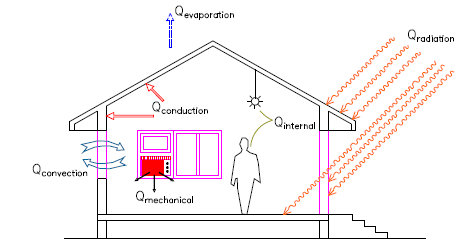
\includegraphics[width=1\textwidth]{figures/HeatTransferProcess}
	\caption{Pertukaran kalor bangunan dengan lingkungan\cite{skripsiIchfan}}
	\label{fig:3:HeatTransferProcess}
\end{figure}

Lingkungan termal bangungan dipengaruhi oleh beberapa faktor. Faktor-faktor tersebut diantaranya geometri bangunan, material bangunan, iklim, dan penggunaan bangunan itu sendiri. Proses perpindahan kalor yang membentuk lingkungan termal secara rinci dibagi menjadi 4 bagian, yaitu:

\begin{enumerate}
	\item Proses perpindahan panas yang terjadi di muka luar dari selubung bangunan
	\item Proses perpindahan panas yang terjadi di selubung bangunan
	\item Proses perpindahan panas yang terjadi di muka dalam dari selubung bangunan
	\item Proses perpindahan panas dan massa yang terjadi di udara dalam bangunan
\end{enumerate}

\noindent Keempat proses perpindahan kalor ini diringkas pada Gambar \ref{fig:3:HeatTransferScheme}.

\begin{figure}[!h]
	\centering
	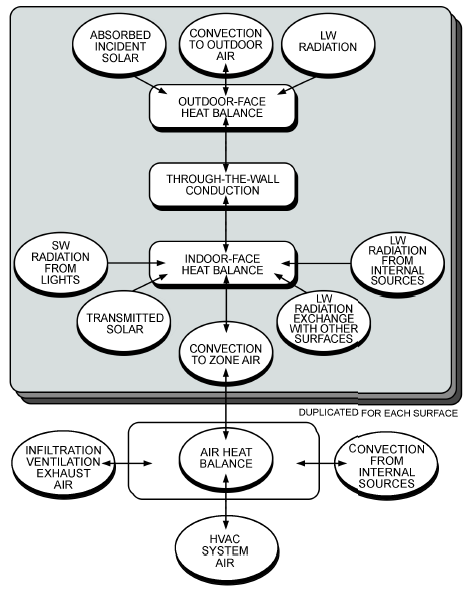
\includegraphics[width=0.8\textwidth]{figures/HeatTransferScheme}
	\caption{Skema keseimbangan proses perpindahan panas dalam bangunan\cite{skripsiIchfan}}
	\label{fig:3:HeatTransferScheme}
\end{figure}

\subsection{Kenyamanan Termal}
Kenyamanan termal adalah suatu kondisi pikiran yang mengekspresikan kepuasan dengan lingkungan termal, baik secara fisiologis maupun psikologis, dan dinilai dengan evaluasi subyektif oleh penghuni itu sendiri \cite{ASHRAE55}. Kenyamanan termal penting untuk kesehatan dan kebugaran tubuh manusia. Hal tersebut berpengaruh terhadap produktivitas manusia dalam melakukan kegiatan. Kurangnya kenyamanan termal dapat mengakibatkan kondisi stres bagi penghuni bangunan. Apabila kondisi bangungan terlalu panas, maka penghuni akan merasa lelah. Apabila kondisi bangunan terlalu dingin, maka penghuni akan merasa gelisah dan bimbang. Dalam hal sensasi, kenyamanan termal digambarkan sebagai sensasi termal dalam bentuk \textit{too warm} atau \textit{too cold}, yang ditentukan oleh skala tujuh poin sensasi termal berdasarkan ASHRAE sebagai berikut:

\qquad\qquad\qquad\qquad\qquad\qquad -3 = cold

\qquad\qquad\qquad\qquad\qquad\qquad -2 = cool

\qquad\qquad\qquad\qquad\qquad\qquad -1 = slightly cool

\qquad\qquad\qquad\qquad\qquad\qquad\ 0 = neutral

\qquad\qquad\qquad\qquad\qquad\qquad\ 1 = slightly warm

\qquad\qquad\qquad\qquad\qquad\qquad\ 2 = warm

\qquad\qquad\qquad\qquad\qquad\qquad\ 3 = hot


Standar SNI terkait kenyamanan termal ruangan, yaitu menjaga suhu dan kelembapan ruangan pada nilai tertentu. Nilai standar suhu ruang (\textit{drybulb}) dijaga pada nilai $25\pm 1^{\circ}C$, dan nilai kelembapan dalam bentuk \textit{relative humidity} (RH), dijaga pada nilai $60\% \pm 10\%$ untuk kenyamanan penghuni \cite{SNI-03-06390-2000}.

\section{Kontrol Otomatis}

Kontrol otomatis telah memegang peranan yang sangat penting dalam perkembangan ilmu dan teknologi. Di samping sangat diperlukan pada pesawat ruang angkasa, peluru kendali, sistem kontrol pesawat, dan sebagainya, sistem kontrol juga mejadi bagian penting dan terpadu dari proses-proses dalam pabrik dan industri modern. Sistem kontrol otomatis sangat diperlukan dalam operasi-operasi di industri untuk mengendalikan tekanan, temperatur, laju aliran dan sebagainya.

\subsection{Dasar-dasar Ilmu Kontrol}

Sistem adalah kombinasi dari beberapa komponen yang bekerja bersama-sama dan bersinergi untuk mencapai tujuan yang diinginkan. Sistem tidak hanya dibatasi hanya untuk sistem fisik saja. Konsep sistem dapat digunakan pada gejala yang abstrak dan dinamis lainnya seperti sistem ekonomi, biologi, organisasi, dan lain sebagainya. Sistem kontrol adalah interkoneksi dari berbagai komponen kontrol yang membentuk suatu konfigurasi sistem yang akan menghasilkan respon sistem yang diinginkan.

Komponen utama dari sistem kontrol terdiri dari proses dan kontroler. Proses adalah komponen atau grup yang terdiri dari beberapa komponen yang dikendalikan. Kontroler adalah komponen yang mengendalikan proses. Keluaran dari kontroler adalah nilai variabel yang memanipulasi proses.

Sistem kontrol dapat dikategorikan menjadi dua macam, yakni sistem kontrol kalang terbuka dan sistem kontrol kalang tertutup. Sistem kontrol kalang terbuka adalah sistem kontrol yang keluarannya tidak berpengaruh pada aksi kontrol. Pada sistem ini keluaran tidak dibandingkan dengan \textit{setpoint}. Dengan demikian, setiap \textit{setpoint} memiliki suatu kondisi operasi yang tetap. Jadi ketelitian sistem tergantung dari kalibrasi sistem. Sistem kontrol kalang terbuka ini juga tidak akan bisa bekerja jika ada gangguan internal maupun eksternal pada sistem. Sistem kontrol kalang tertutup atau sistem kontrol berumpan balik adalah sistem kontrol yang sinyal keluarannya mempunyai pengaruh langsung pada aksi kontrol. Sinyal kesalahan penggerak, yang merupakan selisih antara nilai keluaran sistem dan nilai \textit{setpoint} diumpankan ke kontroler untuk memperkecil kesalahan dan membuat agar nilai keluaran sistem mendekati harga yang diinginkan (\textit{setpoint}). Penggunaan umpan balik membuat respon sistem menjadi kurang peka terhadap gangguan internal maupun eksternal. Sehingga, jika dibandingkan dengan sistem kontrol kalang terbuka, sangat mungkin diperoleh sistem kontrol yang lebih teliti meskipun menggunakan komponen-komponen yang relatif kurang teliti. \cite{ControlSystemBook}

Sistem kontrol merupakan hal yang dinamis. Sistem akan memberikan respon terhadap input yang diberikan, dimana pada awalnya sistem akan memberikan suatu respon transien yang selanjutnya tercapai kondisi keadaan-ajeg yang secara umum akan mengikuti input yang diberikan. Terdapat tiga hal utama tujuan desain dan analisis dari sistem kontrol, yaitu: \cite{ControlSystemBook}
\begin{enumerate}
	\item Menghasilkan spesifikasi dari respon transien yang diinginkan.
	\item Mengurangi kesalahan pada keadaan-ajeg.
	\item Mencapai kestabilan sistem.
\end{enumerate}

\noindent \textbf{Respon Transien}

Jika suatu sistem kontrol dikenakan suatu input tertentu, sistem tidak dapat langsung mengikuti input yang diberikan, tetapi sistem terlebih dahulu akan berusaha untuk menyesuaikan karakter naturalnya dengan input yang diberikan. Respon inilah yang dinamakan respon transien dan menjadi hal penting untuk dianalisis dalam desain sistem kontrol. Sebagai contoh adalah respon sistem kontrol posisi elevator. Jika respon transien terlalu lambat maka akan membuat penumpang tidak sabar. Tetapi jika respon transien terlalu cepat maka akan membuat penumpang merasa tidak nyaman. Respon transien juga penting untuk alasan struktur. Respon transien yang terlalu cepat dapat juga menyebabkan kerusakan fisik pada peralatan yang dikendalikan.\cite{ControlSystemBook} \\

\noindent \textbf{Respon Keadaan-Ajeg}

Salah satu tujuan dari desain dan analisis dari sistem kontrol difokuskan pada respon keadaan-ajeg. Misalnya dalam sistem kontrol posisi elevator, kesalahan pada keadaan-ajeg akan menyebabkan posisi elevator tidak tepat pada lantai yang dituju, tetapi mungkin pada posisi di atas atau di bawahnya. Dalam keadaan-ajeg diharapkan respon sistem sesuai dengan input yang diberikan. Tujuan dari desain dan analisis sistem kontrol diarahkan pada bagaimana memperkecil kesalahan pada keadaan-ajeg.\cite{ControlSystemBook} \\

\noindent \textbf{Kestabilan Sistem}

Respon dari sistem merupakan hasil penjumlahan dari respon natural sistem dan respon paksaan. Respon natural merupakan respon sistem karena karakter natural dari sistem. Respon paksaan adalah respon sistem terhadap input atau paksaan yang diberikan pada sistem.
Sistem kontrol dikatakan stabil jika respon natural:
\begin{enumerate}
	\item Pada rentang tertentu bernilai mendekati nol, sehingga hanya menyisakan respon paksaan, atau
	\item berosilasi.
\end{enumerate}

Jika respon natural dari sistem membesar sehingga lebih besar dari respon paksaannya, maka sistem dikatakan tidak stabil. Hal ini bisa mengakibatkan kondisi-kondisi yang tidak menguntungkan. Misalnya, suatu elevator akan meluncur sampai menembus atap, posisi antena akan terus berputar dan sebagainya.\\

\noindent\textbf{Proses Pengendalian}

Proses pengendalian merupakan tugas seorang insinyur kontrol untuk menganalisis sistem yang ada, dan merancang sistem baru untuk memenuhi kebutuhan spesifik. Terkadang sistem baru perlu dirancang, tetapi suatu unit kontroler lebih sering dirancang untuk meningkatkan kinerja sistem yang ada. Ketika perancangan suatu sistem atau penerapan suatu kontroler dalam menambah sistem yang ada, perlu mengikuti beberapa langkah berikut: \cite{ControlSystemBook}
\begin{enumerate}
	\item Pemodelan sistem
	\item Analisis sistem
	\item Perancangan kontroler
	\item Penerapan kontroler dan pengujian
\end{enumerate}

\subsection{Kesalahan Keadaan-Ajeg}

Kesalahan keadaan-ajeg adalah perbedaan antara input dan output untuk input tes yang ditentukan ketika $t \rightarrow \infty$. Dalam sistem kontrol, diperhatikan perbedaan antara input dan output dari sistem kontrol umpan balik setelah mencapai keadaan-ajeg. Dengan demikian, hal ini dibatasi untuk sistem yang stabil, dimana respons alami mendekati nol selayaknya $t \rightarrow \infty$ . Sistem yang tidak stabil merepresentasikan hilangnya kendali dalam keadaan-ajeg dan sama sekali tidak dapat diterima untuk digunakan. Persamaan yang diperoleh untuk menghitung kesalahan keadaan-ajeg dapat diterapkan secara keliru ke sistem yang tidak stabil. Dengan demikian, insinyur harus memeriksa stabilitas sistem saat melakukan analisis dan perancangan kesalahan keadaan-ajeg.

Banyak kesalahan keadaan-ajeg pada sistem kontrol muncul dari sumber nonlinear, seperti serangan balik dari roda gigi atau motor yang tidak bergerak terkecuali ketika tegangan input melebihi nilai ambang batas. Kesalahan keadaan-ajeg yang dipelajari adalah kesalahan yang muncul dari konfigurasi sistem itu sendiri dan jenis input yang diterapkan. 

\begin{figure}[!h]
	\centering
	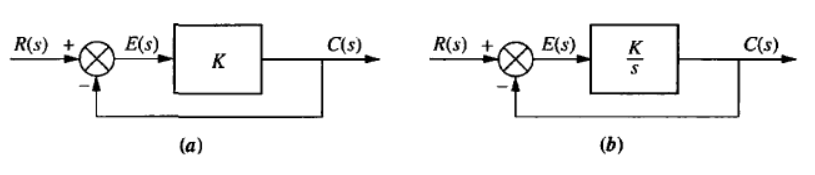
\includegraphics[width=0.75\textwidth]{figures/SSEExample}
	\caption{Sistem dengan \textbf{a.} kesalahan keadaan-ajeg bernilai terbatas untuk input fungsi step; \textbf{b.} kesalahan keadaan-ajeg nol untuk input fungsi step \cite{ControlSystemBook}}
	\label{fig:3:steadystateerror}
\end{figure}

Contohnya, amati Gambar \ref{fig:3:steadystateerror}(a), dimana $R(s)$ adalah input, $C(s)$ adalah output, dan $E(s) = R(s) - C(s)$ adalah galat (kesalahan keadaan-ajeg). Pada keadaan-ajeg, jika $c(t) = r(t)$, maka $e(t)$ bernilai nol. Tetapi dengan adanya \textit{gain} (pengali) $K$, galat tersebut, $e(t)$, tidak dapat bernilai nol jika $c(t)$ bernilai terbatas dan tak nol. Sehingga, keutamaan dari konfigurasi sistem (\textit{gain} murni K pada umpan maju), haruslah memiliki nilai galat. Jika kita sebut $c_{steady-state}$ adalah nilai keadaan-ajeg suatu output dan $e_{steady-state}$ adalah nilai keadaan-ajeg suatu galat, maka $c_{steady-state} = K e_{steady-state}$, atau 

\begin{equation} \label{eq:3:steady-state-error}
e_{steady-state} = \frac{1}{K} \ c_{steady-state}
\end{equation}

Dengan demikian, semakin besar nilai K dan semakin kecil nilai $e_{steady-state}$ haruslah menghasilkan nilai $c_{steady-state}$ yang sama. Kesimpulan yang dapat kita tarik yaitu \textit{gain} murni pada umpan maju akan selalu menjadi suatu kesalahan keadaan-ajeg untuk input fungsi step. Kesalahan ini berkurang ketika nilai K meningkat.

%Jika penguatan jalur maju digantikan oleh integrator, seperti yang ditunjukkan pada Gambar \ref{fig:3:steadystateerror}(b), akan ada nol kesalahan pada kondisi ajeg untuk input fungsi steo. Alasannya adalah sebagai berikut: Ketika $c(t$ meningkat, $e(t)$ akan berkurang, karena $e(t) = r(t) - c(t)$. Penurunan ini akan berlanjut hingga tidak ada kesalahan nol, tetapi masih akan ada nilai untuk $c(t)$ karena integrator dapat memiliki output yang konstan tanpa input apa pun. Misalnya, motor dapat direpresentasikan hanya sebagai integrator. Tegangan yang diberikan pada motor akan menyebabkan putaran. Ketika tegangan yang diberikan dilepas, motor akan berhenti dan tetap pada posisi keluaran saat ini. Karena tidak kembali ke posisi semula, kami memiliki output perpindahan sudut tanpa input ke motor. Oleh karena itu, sistem yang mirip dengan Gambar \ref{fig:3:steadystateerror}(b), yang menggunakan motor di jalur maju, dapat memiliki nol kondisi ajeg untuk input fungsi step \cite{ControlSystemBook}.

%\begin{figure}[!h]
%	\centering
%	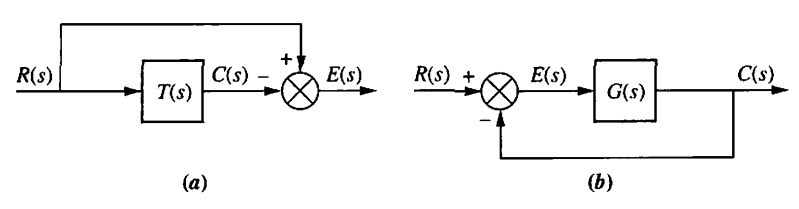
\includegraphics[width=0.75\textwidth]{figures/SSEExample2}
%	\caption{Galat sistem kontrol tertutup: a. Representasi secara umum; b. Representasi untuk sistem umpan balik satuan}
%	\label{fig:3:steadystateerror2}
%\end{figure}

%Pertimbangkan Gambar \ref{fig:3:steadystateerror2}(a). Untuk menentukan $E(s)$, kesalahan antara input, $R(s)$, dan output, $C(s)$, ditulis sebagai:
%\begin{equation} \label{eq:3:steady-state-error2}
%E(s) = R(s) - C(s)
%\end{equation}
%tetapi,
%\begin{equation} \label{eq:3:steady-state-error3}
%C(s) = R(s)T(s)
%\end{equation}
%Dengan mensubstitusi Persamaan \ref{eq:3:steady-state-error3} ke \ref{eq:3:steady-state-error2}, lalu disederhanakan dan dicari solusi pemecahan untuk $E(s)$, yaitu:
%\begin{equation} \label{eq:3:steady-state-error4}
%E(s) = R(s)(1 - T(s))
%\end{equation}
%Meskipun Persamaan \ref{eq:3:steady-state-error4} membantu kita dalam menyelesaikan $e(t)$ di setiap waktu, t, tetapi kita lebih tertarik untuk mengetahui nilai akhir dari galat, $e(\infty)$. Dengan mengaplikasikan teorema nilai akhir, yang mana memungkinkan kita untuk menggunakan nilai akhir dari $e(t)$ tanpa mengambil transformasi balik Laplace $E(S)$, dan kemudian membiarkan $t$ mendekati $\infty$, didapatkan
%\begin{equation} \label{eq:3:steady-state-error5}
%e(\infty) = \lim_{t \to \infty} e(t) = \lim_{s \to 0} sE(s)
%\end{equation}
%Substitusi Persamaan \ref{eq:3:steady-state-error4} ke \ref{eq:3:steady-state-error5}, didapatkan:
%\begin{equation} \label{eq:3:final-steady-state-error}
%e(\infty) = \lim_{t \to \infty} e(t) = \lim_{s \to 0} sR(s)[1 - T(s)]
%\end{equation}

%Pertimbangkan sistem kontrol umpan balik ditunjukkan pada Gambar \ref{fig:3:steadystateerror2}(b). Karena umpan balik, $H(s)$, sama dengan 1, sistem memiliki umpan balik satuan. Implikasinya adalah bahwa $E(s)$ sebenarnya adalah kesalahan antara input, $R(s)$, dan output, $C(s)$. Jadi, jika kita memecahkan Persamaan untuk $E(s)$, kita akan memiliki ekspresi untuk kesalahan tersebut. Kemudian diterapkan teorema nilai akhir untuk mengevaluasi kesalahan keadaan-ajeg.

%Menulis $E(s)$ berdasarkan Gambar \ref{fig:3:steadystateerror2}(b), didapatkan
%\begin{equation} \label{eq:3:sse-g}
%E(s) = R(s) - C(s)
%\end{equation}
%Tetapi,
%\begin{equation} \label{eq:3:sse-g2}
%C(s) = E(s)G(s)
%\end{equation}
%Substitusi Persamaan \ref{eq:3:sse-g2} ke \ref{eq:3:sse-g}, didapatkan:
%\begin{equation} \label{eq:3:sse-g3}
%E(s) = \frac{ R(s) }{ 1 + %G(s) }
%\end{equation}
%Kemudikan diterapkan teorema nilai akhir, \ref{eq:3:steady-state-error5}. Pada titik ini dalam perhitungan numerik, kita harus memeriksa apakah sistem loop tertutup stabil, menggunakan, misalnya, kriteria Routh-Hurwitz. Namun, untuk saat ini, asumsikan bahwa sistem loop tertutup adalah stabil dan gantikan Persamaan \ref{eq:3:sse-g3} ke Persamaan \ref{eq:3:steady-state-error5}, didapatkan:
%\begin{equation} \label{eq:3:sse-g4}
%e(\infty) = \lim_{s \to 0} \frac{ sR(s) }{ 1 + G(s) }
%\end{equation}


\section{Jaringan Saraf Tiruan}
Jaringan Saraf Tiruan (JST) dimodelkan dengan mengadaptasi proses biologis untuk pemrosesan informasi, termasuk secara khusus sistem saraf dan unit dasarnya, neuron (sel saraf). Sinyal didistribusikan dalam bentuk beda potensial antara bagian dalam dan luar sel. Komponen sel saraf (neuron) ditunjukkan pada Gambar \ref{fig:3:neuron}. Dendrit membawa sinyal dari neuron lain ke dalam badan sel (soma), kemungkinan dengan memperkalikan setiap sinyal yang masuk dengan koefisien pembobotan pengiriman.\cite{NNControlBook}

\begin{figure}[!h]
	\centering
	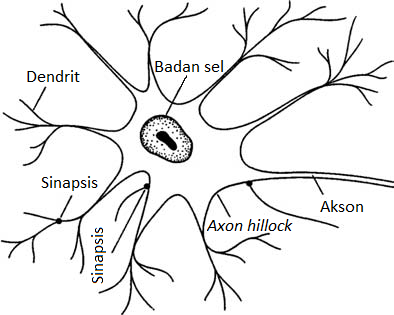
\includegraphics[width=0.75\textwidth]{figures/neuron}
	\caption{Anatomi neuron \cite{NNControlBook}}
	\label{fig:3:neuron}
\end{figure}

Pada badan sel, kapasitansi sel mengintegrasikan sinyal yang terkumpul di \textit{axon hillock} (bagian khusus dari badan sel neuron yang terhubung dengan akson). Sekalinya sinyal gabungan melebihi ambang batas nilai tertentu, sinyal/impuls ditransmisikan melalui akson. Ketidaklinieran sel menjadikan impuls komposit sebagai fungsi nonlinier dari kombinasi sinyal yang datang. Akson tersebut, melalui sinapsis, terhubung dengan dendrit pada neuron berikutnya. Sinapsis beroperasi melalui pelepasan kimiawi \textit{neurotransmitter} melintasi celah antar sel, dan dapat berupa \textit{excitatory} (kecenderungan dalam pengaktifan neuron berikutnya) atau \textit{inhibitory} (kecenderungan dalam mencegah pengaktifan neuron berikutnya) \cite{NNControlBook}.

\begin{figure}[!h]
	\centering
	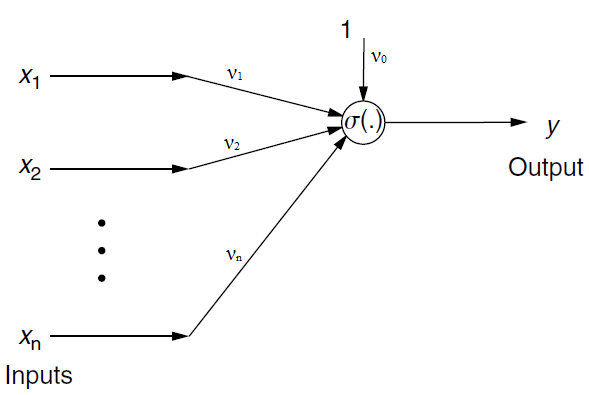
\includegraphics[width=0.75\textwidth]{figures/neuronmath}
	\caption{Model matematis neuron \cite{NNControlBook}}
	\label{fig:3:math}
\end{figure}

\subsection{Model Matematis Neuron}

Model matematis dari suatu neuron dilukiskan oleh Gambar \ref{fig:3:math}, yang mana menunjukkan pembobotan dendrit $v_j$, nilai ambang batas $v_0$ (disebut juga sebagai bias), penjumlahan dari sinyal masuk yang diberi bobot, dan fungsi nonlinear $\sigma(\cdot)$. Sel input adalah sinyal ke-$n$ pada waktu instan 	$kx_1(k), kx_2(k), kx_3(k),...,x_n(k)$ dan outputnya adalah nilai skalar $y(k)$, yang dapat dinyatakan sebagai

\begin{equation} \label{eq:3:perceptron}
y(k) = \sigma \left( \sum_{j=1}^{n}v_jx_j(k)+v_0 \right)
\end{equation}

Bobot-bobot positif  $v_j$ berhubungan dengan sinapsis \textit{exitatory} dan bobot-bobot negatif dengan sinapsis \textit{inhibitory}. Jaringan ini disebut sebagai \textit{perceptron} oleh Rosenblatt pada tahun 1959.

Fungsi sel nonlinear dikenal sebagai fungsi aktivasi. Fungsi aktivasi dipilih secara khusus untuk aplikasi-aplikasi meskipun beberapa pilihan yg umum diilustrasikan pada Gambar \ref{fig:3:activation}. Intensi pada fungsi aktivasi adalah untuk memodelkan perilaku nonlinier suatu sel dimana tidak terdapat output di bawah nilai tertentu suatu argumen. Fungsi sigmoid adalah sebuah kelas umum dari fungsi yang tidak meningkat secara monoton dengan mengambil nilai-nilai yang dibatasi antara nilai $-\infty$ dan $+\infty$. 
\begin{figure}[!h]
	\centering
	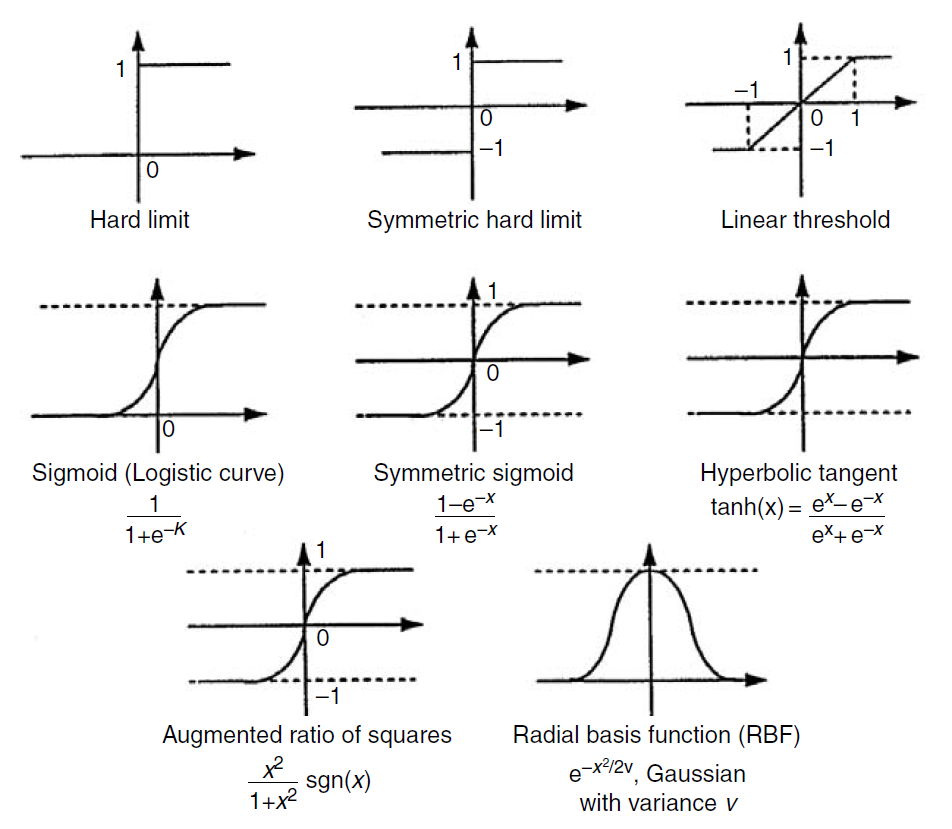
\includegraphics[width=1\textwidth]{figures/activationFunction}
	\caption{Fungsi-fungsi aktivasi \cite{NNControlBook}}
	\label{fig:3:activation}
\end{figure}
Perlu dicatat bahwa ketika nilai ambang batas atau bias $v_0$ berubah, fungsi aktivasi bergeser ke kiri atau ke kanan. Untuk kebanyakan algoritma pelatihan JST (termasuk \textit{backpropagation}), turunan dari $\sigma(\cdot)$ dibutuhkan sehingga fungsi aktivasi yang dipilih haruslah dapat terdiferensiasi.\cite{NNControlBook}

Ekspresi untuk output neuron $y(k)$ pada waktu instan $k$ (dalam kasus waktu yang kontinyu) dapat dirampingkan dengan menentukan vektor kolom dari bobot-bobot JST $\ \overline{v}(k) \in \mathbb{R}^n $ sebagai
\vspace{-1em}
\begin{equation} \label{eq:3:vektorKolom}
\overline{x}(k) = [x_1\ x_2\ \cdots\ x_n]^T, \qquad \overline{v}(k) = [v_1\ v_2\ \cdots\ v_n]^T
\end{equation}

Kemudian, ini memungkinkan untuk ditulis dalam notasi matriks
\vspace{-1em}
\begin{equation} \label{eq:3:matriksy}
y = \sigma(\overline{v}^T\overline{x}) + v_0
\end{equation}

Vektor kolom input \textit{augmented} $x(k) \in \mathbb{R}^{n+1} $ dan vektor kolom bobot JST $v(k) \in \mathbb{R}^{n+1} $ didefinisikan sebagai
\vspace{-1em}
\begin{equation} \label{eq:3:matriksaugmented}
\begin{split}
x(k) = [1\;\; \overline{x}^T]^T = [1\;\; x_1\ x_2\ \cdots\ x_n]^T \\
v(k) = [v_0\ \overline{v}^T]^T = [v_0\ v_1\ v_2\ \cdots\ v_n]^T
\end{split}
\end{equation}

yang dapat juga ditulis sebagai
\vspace{-2em}
\begin{equation} \label{eq:3:matriksfinal}
\begin{split}
y = \sigma(v^Tx)
\end{split}
\end{equation}

\begin{figure}[!h]
	\centering
	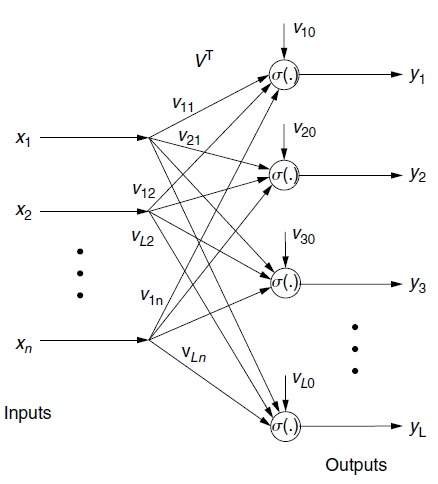
\includegraphics[width=0.75\textwidth]{figures/jstTunggal}
	\caption{Jaringan layar tunggal \cite{NNControlBook}}
	\label{fig:3:jstTunggal}
\end{figure}
Meskipun vektor input $\overline{x}(k) \in \mathbb{R}^n $ dan vektor bobot $\overline{v}(k) \in \mathbb{R}^n $ masing-masing telah ditambahkan dengan 1 dan $v_0$, untuk memasukkan nilai bias, terkadang dengan bebas dapat dinyatakan bahwa $x(k)$ dan $v$ adalah elemen $\mathbb{R}^n$.

Vektor penggambaran output neuron $y(k)$ disebut sebagai mekanisme penarikan sel. Vektor tersebut mendeskripsikan bagaimana output itu direkonstruksi dari sinyal input dan nilai parameter sel.

Gambar \ref{fig:3:jstTunggal} menunjukkan sebuah JST yang mengandung L buah sel, semuanya diberi umpan oleh sinyal input yang sama dan memproduksi satu output $y(k)$ per neuron. Hal ini disebut sebagai jaringan layar tunggal. Persamaan \textit{recall} untuk jaringan ini ditunjukkan sebagai berikut
\vspace{0em}
\begin{equation} \label{eq:3:recall}
y_l(k) = \sigma \left( \sum_{j=1}^{n}v_{lj}x_j(k)+v_{l0} \right); \qquad l = 1,2,...,L
\end{equation}

Akan lebih mudah untuk menulis bobot dan bias masing-masing dalam bentuk matriks dan vektor. Dengan menentukan matriks bobot dan vektor bias sebagai berikut
\vspace{-1em}
\begin{equation} \label{eq:3:weightVector}
\overline{V}^T \equiv
\left[
\begin{matrix}
v_{11} & v_{12} & \cdots & v_{1n} \\
v_{21} & v_{22} & \cdots & v_{2n} \\
\vdots & \vdots & \ddots & \vdots \\
v_{L1} & v_{L2} & \cdots & v_{Ln} \\
\end{matrix}
\right], \qquad
b_v = 
\left[
\begin{matrix}
v_{10} \\
v_{20} \\
\vdots \\
v_{L0} \\
\end{matrix}
\right],
\end{equation}

\noindent Salah satu cara menulis vektor output $y(t) = [y_0\ y_1\ y_2\ \cdots y_L]^T$ sebagai berikut
\vspace{-1em}
\begin{equation} \label{eq:3:outputVector}
y = \overline{\sigma}(\overline{V}^T\overline{x}+b_v)
\end{equation}
\noindent Vektor fungsi aktivasi yang ditentukan oleh vektor $w\equiv [w_1\ w_2\ \cdots w_L]^T$ adalah
\vspace{-1em}
\begin{equation} \label{eq:3:activation}
\overline{\sigma}(w)\equiv [\overline{\sigma}(w)_1\ \overline{\sigma}(w)_2\ \cdots\ \overline{\sigma}(w)_L]^T
\end{equation}

Penyempurnaan lebih lanjut dapat dicapai dengan memasukkan vektor bias sebagai kolom pertama dari matriks \textit{augmented} bobot sebagai berikut
\vspace{-1em}
\begin{equation} \label{eq:3:fullVector}
V^T \equiv
\left[
\begin{matrix}
v_{10} & v_{11} & \cdots & v_{1n} \\
v_{20} & v_{21} & \cdots & v_{2n} \\
\vdots & \vdots & \ddots & \vdots \\
v_{L0} & v_{L1} & \cdots & v_{Ln} \\
\end{matrix}
\right]
\end{equation}\

Kemudian output JST dapat digambarkan dalam bentuk vektor \textit{augmented} input $x(k)$ sebagai
\vspace{0em}
\begin{equation} \label{eq:3:finalVector}
y = \overline{\sigma}(V^Tx)
\end{equation}

\subsection{Jaringan Layar Jamak (MLP)}
Jaringan layar jamak (\textit{Multilayer Perceptron}) merupakan perluasan dari jaringan layar tunggal (\textit{perceptron}). Sebuah JST 2 layar memiliki dua lapisan neuron dengan satu layar memiliki $L$ buah neuron yang memberikan umpan kepada lapisan kedua yang memiliki $m$ buah neuron, digambarkan pada Gambar \ref{fig:3:mlp}. Lapisan pertama dikenal sebagai lapisan tersembunyi, dengan $L$ sebagai jumlah neuron pada lapisan tersembunyi tersebut. Lapisan kedua dikenal sebagai lapisan output. Jaringan saraf tiruan yang terdiri dari banyak lapisan disebut sebagai \textit{multilayer perceptron}. Daya komputasi untuk lapisan ini perlu ditingkatkan secara signifikan dibandingkan jaringan layar tunggal. Dengan jaringan layar tunggal, dimungkinkan untuk menerapkan operasi digital seperti AND, OR, dan COMPLEMENT. 
\begin{figure}[!h]
	\centering
	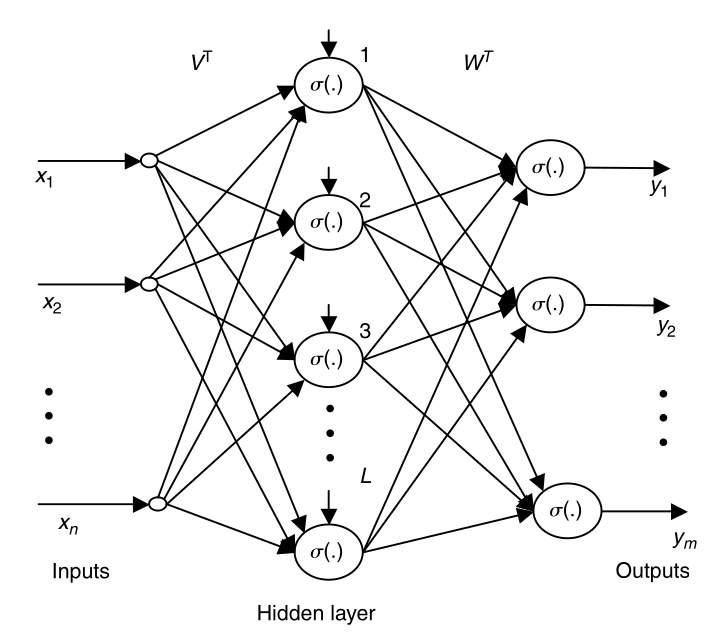
\includegraphics[width=0.75\textwidth]{figures/mlp}
	\caption{Jaringan 2 layar \cite{NNControlBook}}
	\label{fig:3:mlp}
\end{figure}
Namun, penelitian mengenai JST telah dihentikan bertahun-tahun yang lalu ketika ditunjukkan bahwa jaringan layar tunggal tidak mampu melakukan operasi EXCLUSIVE OR (X-OR), yang merupakan masalah dasar dalam perancangan sistem logika digital. Kemudian telah ditunjukkan bahwa jaringan 2 layar dapat menerapkan operasi EXCLUSIVE OR (X-OR) dan ini kembali mempercepat penelitian JST di awal 1980-an. Beberapa peneliti (Hush dan Horne 1993) mempresentasikan solusi untuk operasi X-OR dengan menggunakan fungsi aktivasi sigmoid.

\noindent Output jaringan 2 layar ditunjukkan oleh Persamaan \textit{recall} berikut
\begin{equation} \label{eq:3:2layerOut}
y_i = \sigma
\left(
\sum_{l=1}^{L}w_{il}\sigma
	\left(
		\sum_{j=1}^{n}v_{lj}x_j + v_{l0}
	\right)
	+ w_{i0}
\right); \qquad i = 1,2,\dots,m
\end{equation}

\noindent Menentukan output jaringan tersembunyi $z_1$ dapat ditulis sebagai berikut
\begin{equation} \label{eq:3:hiddenlayer}
\begin{split}
z_l = \sigma\left(\sum_{j=1}^{n}v_{lj}x_j+v_{l0} \right);\qquad l = 1,2,\dots,L\\
y_i = \sigma\left(\sum_{l=1}^{L}w_{il}z_l+w_{i0} \right);\qquad l = 1,2,\dots,m
\end{split}
\end{equation}

\noindent Menentukan matriks bobot layar pertama $\overline{V}$ dan $V$ dan matriks bobot layar kedua sebagai berikut
\begin{equation} \label{eq:3:weight21Vector}
\overline{W}^T \equiv
\left[
\begin{matrix}
w_{11} & w_{12} & \cdots & w_{1n} \\
w_{21} & w_{22} & \cdots & w_{2n} \\
\vdots & \vdots & \ddots & \vdots \\
w_{L1} & w_{L2} & \cdots & w_{Ln} \\
\end{matrix}
\right], \qquad
b_w = 
\left[
\begin{matrix}
w_{10} \\
w_{20} \\
\vdots \\
w_{L0} \\
\end{matrix}
\right],
\end{equation}
\begin{equation} \label{eq:3:weight22Vector}
W^T \equiv
\left[
\begin{matrix}
w_{10} & w_{11} & \cdots & w_{1n} \\
w_{20} & w_{21} & \cdots & w_{2n} \\
\vdots & \vdots & \ddots & \vdots \\
w_{L0} & w_{L1} & \cdots & w_{Ln} \\
\end{matrix}
\right]
\end{equation}

\noindent Output JST dapat ditulis sebagai berikut
\begin{equation} \label{eq:3:2layer}
y = \overline{\sigma}
\left(
	\overline{W}^T\overline{\sigma}(\overline{V}^T\overline{x}+b_v)+b_w
\right),
\end{equation}
atau
\begin{equation} \label{eq:3:2layerfinal}
y = \overline{\sigma}
\left(
	W^T\sigma(V^Tx)
\right).
\end{equation}
Pada Persamaan ini, notasi $\overline{\sigma}$ berarti bahwa vektor ditentukan sesuai dengan Persamaan (\ref{eq:3:activation}). Dalam (\ref{eq:3:2layerfinal}) perlu menggunakan vektor \textit{augmented}
\begin{equation} \label{eq:3:augVector}
\sigma(w) \equiv [1\quad \overline{\sigma}(w)^T]^T = [1\quad \sigma(w_1)\ \sigma(w_2)\ \dots\ \sigma(w_L)\ ]^T,
\end{equation}
\noindent dimana nilai 1 ditempatkan sebagai entri pertama untuk memungkinkan penggabungan bias $w_{i0}$ sebagai kolom pertama dari $W^T$. Dalam hal vektor output layar tersembunyi $z\in \mathbb{R}^L$ seseorang dapat menuliskan
\begin{equation} \label{eq:3:final19}
\overline{z} = \sigma(V^Tx),
\end{equation}
\begin{equation} \label{eq:3:final20}
y = \sigma(W^Tz).
\end{equation}
\noindent dimana $z \equiv [1\quad \overline{z}^T]^T$

\break
\break
\break
\break

\section{Kontrol Jaringan Saraf Tiruan}

Untuk mengendalikan lingkungan termal, pada umumnya menggunakan sistem kontrol modern (\textit{modern control system}). Hal ini didasarkan pada karakteristik lingkungan termal yang memiliki sifat MIMO (\textit{multiple input multiple output}). Dengan demikian, sistem kontrol klasik tidak tepat digunakan untuk sistem ini.
\begin{table}[!h]
	\caption{Perbandingan metode kontrol \cite{MPCDissertation}}
	\label{tbl:3:whyann}
	\centering
	% use packages: array
	\begin{tabular}{|p{4cm}|p{4cm}|p{4.5cm}|}
		\hline
		\textbf{Metode kontrol} & \textbf{Klasik} & \textbf{Modern} \\ 
		\hline
		Domain & Frekuensi, Domain-S & Waktu, Domain-t \\ 
		\hline
		Representasi Model & Fungsi Transfer & State-Space \\ 
		\hline
		Kontinyuitas & Kontinyu & Kontinyu, Diskrit, \textit{Hybrid} \\ 
		\hline
		Linieritas & Linier & Linier, Nonlinier \\ 
		\hline
		Variansi waktu & \textit{Time-invariant} (TI) & \textit{Time-variant} (TV) \\ 
		\hline
		Dimensi & SISO & MIMO \\ 
		\hline
		Determinisme & Deterministik & Deterministik, Stokastik \\ 
		\hline
		Optimisasi & Tidak & Ya \\ 
		\hline
		Batasan & Tidak & Ya \\ 
		\hline
		Implementasi & Murah, Mudah & Mahal, Kompleks \\ 
		\hline
	\end{tabular}
\end{table}

Pada umumnya, metode kontrol klasik menggunakan perubahan domain dinamika sistem yang digambarkan oleh Persamaan Diferensial Ordiner (PDE) untuk menghindari komplekstias dari solusi PDE domain waktu. PDE dinamika sistem diubah dari domain waktu ke dalam domain frekuensi menggunakan transformasi Fourier atau secara umum menggunakan transformasi Laplace untuk domain frekuensi bilangan kompleks (domain-s), yang ekuivalen dengan transformasi Z untuk waktu diskret. Pada metode kontrol modern, alih-alih mengubah domain lebih baik menggunakan konversi persamaan diferensial orde tinggi ke dalam persamaan orde 1 domain waktu yang disebut sebagai perasamaan keadaan. Selain itu, representasi langsung dan penanganan sistem multi-input multi-output (MIMO) diperbolehkan menggunakan representasi model fungsi keadaan.\cite{MPCDissertation}

Kelemahan utama dari metode klasik adalah, bahwa mereka hanya dapat digunakan untuk mengendalikan sistem \textit{single-input single-output} (SISO), dengan persyaratan pada model sistem untuk menjadi \textit{linear time-invariant} (LTI). Metode klasik memberikan hasil yang memuaskan hanya dalam mengendalikan proses sederhana, tetapi hasil yang tidak memuaskan dalam kontrol sistem yang lebih kompleks.\cite{MPCDissertation}

Pada dasarnya ada banyak sekali metode kontrol yang merupakan bagian dari metode kontrol modern. Metode-metode tersebut dapat dikelompokkan menjadi beberapa sub kategori. Kategori-kategori tersebut digambarkan dalam bentuk gambar taksonomi pada Gambar \ref{fig:3:ControlSystemTaxonomy}. Berdasarkan taksonomi yang digambarkan pada gambar dibawah, dapat dilihat bahwa Jaringan Saraf Tiruan (\textit{Neural networks}) merupakan salah satu metode kontrol modern.

\begin{figure}[!h]
	\centering
	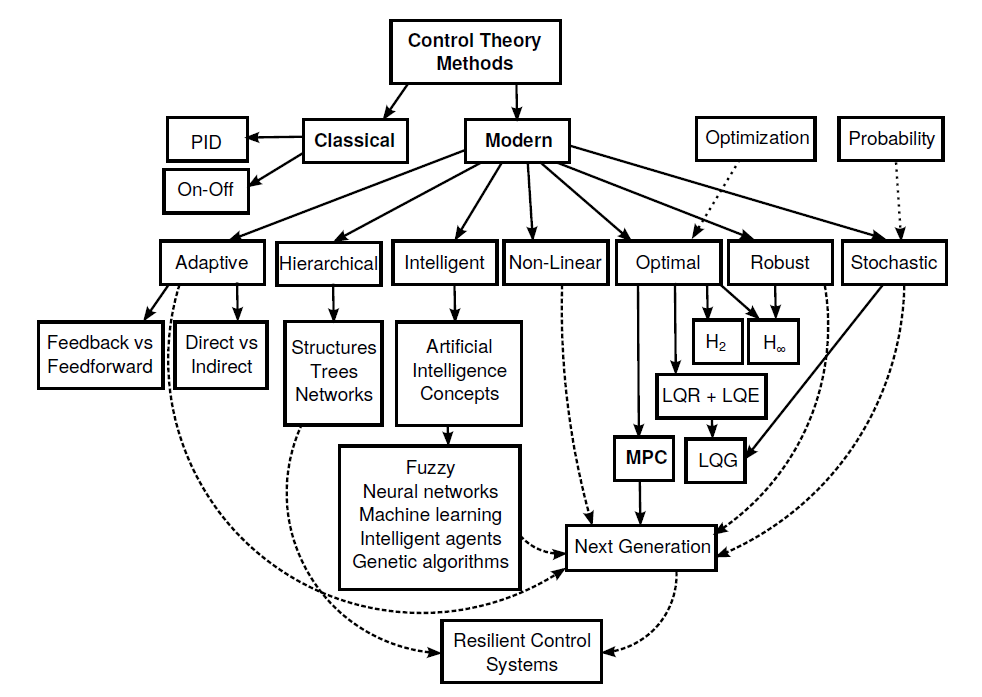
\includegraphics[width=1\textwidth]{figures/ControlSystemTaxonomy}
	\caption{Taksonomi metode kontrok klasik vs modern \cite{NNControlBook}}
	\label{fig:3:ControlSystemTaxonomy}
\end{figure}